\section{Анализ предметной области}

\subsection{Базовые понятия и термины}
Прежде чем приступить к теме исследования, следует описать предмет исследования и связанные с ним термины.
В данной секции описаны понятия, которые будут использоваться в данной работе.

\subsubsection{Ядро Linux}
Ядро Linux — это основной компонент операционной системы Linux, отвечающий за управление ресурсами компьютера и обеспечивающий взаимодействие приложений с аппаратными средствами.\\
Ядро должно в первую очередь выполнять две основные задачи:
\begin{enumerate}
    \item Взаимодействие с аппаратными компонентами, обслуживая все низкоуровневые элементы, входящие в состав аппаратной платформы.
    \item Обеспечить среду выполнения для программ, которые будут выполняться в операционной системе.
\end{enumerate}

Для выполнения данных задача ядро Linux реализует ряд важных архитектурных атрибутов.
Так, например, ядро разделено на несколько отдельных подсистем как на высоком, так и на более низких уровнях.
Данное разделение позволяет упростить разработку и поддержку ядра, а также увеличить его гибкость.
Каждая подсистема ядра реализует свою функциональность, такие как управление памятью, файловой системой, сетевыми интерфейсами, которые могут быть использованы другими подсистемами.
Операционную систему Linux можно считать монолитной системой, поскольку она объединяет все основные службы в одном ядре, что отличает её от микроядерных архитектур, где каждая служба реализуется в отдельном модуле-ядре.\\
При запуске операционной системы ядро загружается в оперативную память компьютера и остается там до тех пор, пока операционная система не будет выключена.
После того, как ядро загружено в оперативную память, ядро выполняет свою инициализацию и начинает планировать задачи.
Когда конкретная задача загружается, ей присваивается виртуальное адресное пространство, в котором она будет находиться.\vspace{0.5cm}\\
\indent Обобщая вышесказанное, можно сказать следующее: ядро решает, какие ресурсы в каком порядке должны быть выделены задаче для её выполнения.
В основном ядро действует как интерфейс между пользовательскими приложениями и оборудованием.\\
Следует отметить, что не все задачи имеют равный доступ к ресурсам компьютера и подсистемам ядра, поскольку в ином случае, например, при возникновении ошибки в одной из задач, она могла бы повредить как другие задачи, так и саму операционную систему.
Безусловно, это далеко не единственная причина, однако, чтобы понять, как ядро определяет к каким ресурсам и подсистемам процессы могут иметь доступ, необходимо для начала представить модель загрузки задач в оперативную память.

\subsubsection{Виртуальная память}\label{subsec:-}

Виртуальная память - это способ организации памяти, при котором процессору предоставляется не физические адреса, а виртуальные адреса, которые в дальнейшем переводятся в физические адреса с помощью таблиц страниц.
\\
Преимущество использования виртуальных адресов заключается в том,
что они позволяют операционной системе управлять представлением памяти,
предоставляемой программному обеспечению.
На практике каждое приложение может использовать свой собственный набор виртуальных адресов,
которые будут отображаться в различных местах физической системы.
Когда операционная система переключается между различными приложениями, она перепрограммирует карту.
Это означает, что виртуальные адреса для текущего приложения будут сопоставлены с правильным физическим расположением в памяти\cite{arm-virt}.\\
%Виртуальные адреса представляют собой набор бит, которые разбиваются на несколько частей: номер страницы, номер сегмента, номер региона\cite{virt-addressing} и номер суперстраницы\cite{superpage}.

\begin{figure}[h]
    \centering
    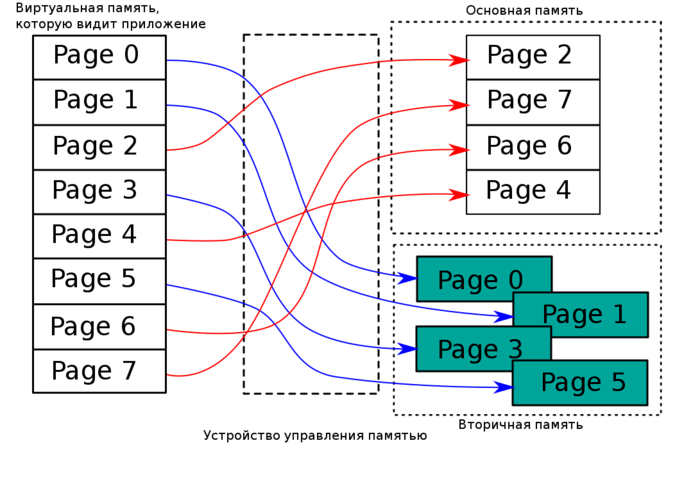
\includegraphics[width=\textwidth]{inc/img/virt_mem}
    \caption{Схема устройства виртуальной памяти}
    \label{fig:virt_mem}
\end{figure}

\newpage

Помимо прочего, для виртуальной памяти были разработаны инструменты для защиты памяти от несанкционированного доступа.
Виртуальная память распределяется на страницы, имеющие фиксированный размер, которые далее распределяются между процессами.
В случае, если процесс попытается получить доступ к странице, которая не принадлежит ему, то процессор сгенерирует исключение, которое будет обработано операционной системой.
\\
Ввиду этого факта, виртуальная память приобретает важное дополнительное свойство.
Различные программы могут быть запущены в отдельных изолированных областях памяти, где они имеют доступ только к тем областям данным,
которые им необходимы для работы.
Отсюда мы переходим к появлению важного двух важных понятий: пространство ядра и пространство пользователя.
\newpage
\subsubsection{Пространство ядра и пространство пользователя}\label{subsec:----}
% FIXME?
Современные операционные системы, в частности Linux, разделяют виртуальную память на пространство ядра и пространство пользователя.
В пространство ядра помещаются само ядро и все необходимые для его работы модули.
Пространство пользователя в свою очередь разделяется на несколько частей.
Каждый процесс получает свое собственное пространство виртуальной памяти, в котором он может хранить свои данные, стек и кучу.
Как было сказано выше, процессы в пространстве пользователя не имеют доступа к чужим областям памяти, однако такой возможностью обладают процессы запущенные в пространстве ядра, которые имеют доступ ко всем областям памяти.
Впервые данная концепция появилась в системе Multics, которая включала в себя 8 <<колец защиты>>\footnotemark, однако в UNIX-системах фактически используются лишь два:
\\
Кольцо 0 - отвечающее за ядро, и кольцо 3 - отвечающее за пользовательские приложения.
\\
Кольца 1 и 2, предоставляемые некоторыми архитектурами процессоров, такие как x86, показали себя неэффективными ввиду сложности портирования на различные архитектуры процессоров, а также ряда других причин.
\\
Схематично данная концепция представлено на рисунке~\ref{fig:rings}.

\footnotetext{Множество современных архитектур процессоров, например Intel x86, переняли эту концепцию и предоставляют 4 кольца защиты на уровне процессора, однако на практике 1-ое и 2-ое кольца практически нигде не используются.}

\begin{figure}[h]
    \centering
    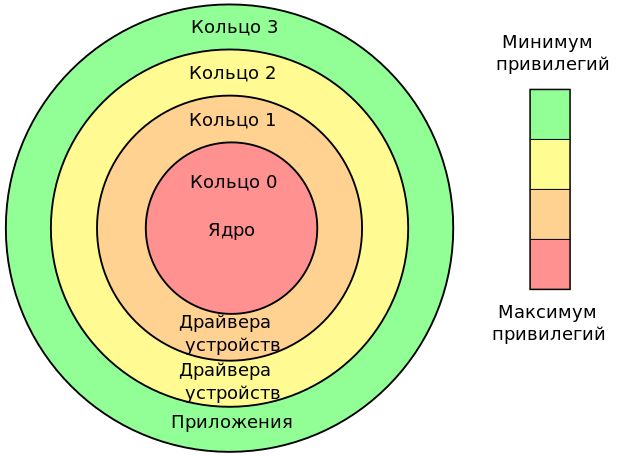
\includegraphics[width=\textwidth]{inc/img/rings}
    \caption{Кольца защиты}
    \label{fig:rings}
\end{figure}

\newpage
% FIXME?

Идея колец защиты заключается в том, что каждое кольцо имеет свой собственный набор инструкций, которые процесс на данном кольце защиты может выполнять, и чем ближе кольцо к нулевому, тем больше прав имеет процесс.
Однако поскольку в UNIX-системах используются лишь два кольца, то далее мы будем к ним относиться как к пространству ядра и пространству пользователя для 0-го и 3-го колец соответственно, пренебрегая остальными.

\subsection{Способы модификации ядра Linux}\label{sec:--anal--methods}

В данной секции будет обозначено, что подразумевается под модификацией ядра Linux для определения в дальнейшем того, какие методы модификации ядра Linux существуют.

\subsubsection{Модификация ядра Linux}\label{subsec:--anal--methods--mod}

В данном разделе описаны основные критерии модификации ядра Linux.

\begin{itemize}
    \item[$-$] \textbf{Модификация ядра Linux} $-$ это изменение кода ядра Linux, которое не включает в себя изменение структуры ядра Linux.
    Таким образом программист волен изменять любые части ядра Linux, не затрагивая саму структуру ядра.
    Любые изменения, которые включают в себя изменение структуры ядра Linux, называются \textbf{переписыванием ядра Linux}, что выходит за рамки данного исследования.
    % FIXME?
    \item[$-$] Главное отличительная особенность модификаций от любых других программ заключается в том, что они работают в пространстве ядра.
    Любой дополнительный функционал, который добавляется в ядро Linux, может оперировать существующими структурами ядра Linux или создавать свои без каких-либо ограничений со стороны ОС.
    \item[$-$] Модификации ядра имеют доступ ко всему функционалу ядра Linux, включая системные вызовы, коммуникацию с устройствами и т.д.
    \item[$-$] Также модификации ядра способны проводить манипуляции в любой области памяти, что позволяет им взаимодействовать с другими модификациями ядра или самим ядром.
\end{itemize}

\subsubsection{Задачи модификации ядра Linux}\label{subsec:---linux}
%  FIXME?
Конкретные задачи модификации ядра крайне обширны и во многом зависят от конкретно поставленной цели конкретного проекта.
Вычисления на уровне ядра дают ряд преимуществ, такие как прямой доступ к оборудованию системы,
ускорение работы программы за счет отсутствия необходимости переключения между пространствами,
возможность манипулировать данными в любой области памяти и т.д.
Однако, в большинстве случаев, такие преимущества либо не являются необходимыми, либо недостатки таких подходов нивелируют эти преимущества.
Общее правило, которое может быть сформировано для всех методов, выглядит следующим образом:
\begin{itemize}
    \item[$-$] Если вычисления на уровне ядра не являются необходимыми, то они не должны быть реализованы.
    \item[$-$] Если вычисления на уровне ядра все же являются необходимыми, то следует провести тщательный анализ, соизмеримое по времени с написанием самой программы, на тему того, не существует ли других альтернатив.
    \item[$-$] Только в том случае, если вычисления на уровне ядра являются необходимыми и других альтернатив не существует, то с особой осторожностью можно приступить к написанию таких программ.
\end{itemize}

Другими словами можно сказать следующее: модификация ядра Linux должна быть последним вариантом,
когда все остальные варианты были исчерпаны.
\\
Следующий список дает примеры некоторых задач, которые должны быть решены на уровне ядра, однако ни в коей мере он не является полным или не лишенным исключений:
%FIXME?
\begin{enumerate}
    \item Написание приложений, таких как драйвера устройств, с доступом к низкоуровневым ресурсам, которые не могут быть предоставлены другими способами.
    \item Реализация алгоритмов, которые должны быть выполнены с высокой точностью по времени и/или пространству (например, мониторинг ресурсов системы или совместное использование ресурсов)\cite{overhead-timer}.
    \item Написание программ, которые должны быть доступны всем пользователям системы.
    \item Также следует перейти в пространство ядра, где накладные расходы, такие как смена пространств пользователь-ядро, становится неприемлемыми для эффективной или корректной работы программы\cite{overhead-timer}.
    Чаще всего в таких случаях мы говорим об облачных вычислениях\cite{overhead-cloud} или любых других вычислениях, требующих высокой производительности.
\end{enumerate}
